% ===========================================================================
\section{Study Area and Data}
\label{sec:data}
% ===========================================================================

\subsection{Nine streams, four provenances}

The nine fuel streams divide into four provenance classes, and the class determines how
much of this paper each stream needs. The metered fossil streams (natural gas, LPG,
kerosene) are read from regulator and industry sales tables and are essentially settled;
the survey-anchored streams (firewood, dung cake, coal, charcoal) take their quantities from
design-weighted HIES microdata; the ledger-derived stream (crop residues, and dung cake
under configuration L) is computed from the agriculture sector's mass balances rather than observed; and the
expenditure-derived generator stream is priced out of the survey's fuel spending. Table
\ref{tab:fuel} gives each stream's energy contribution and source; the rest of this
section treats the streams in declining order of the scrutiny their provenance demands.

\begin{table}[htbp]
\centering
\footnotesize
\begin{tabular}{@{}lrrl@{}}
\toprule
\textbf{Stream} & \textbf{TJ} & \textbf{\%} & \textbf{Source} \\
\midrule
Dung cake     & 126\,827 & 13.6 & HIES rounds, interpolated \\
Firewood      & 360\,873 & 38.7 & HIES 2024--25 quantities \\
Natural gas   & 284\,553 & 30.5 & OGRA domestic sales \\
Crop residues & 122\,192 & 13.1 & Agriculture residue ledger \\
LPG           &  33\,948 &  3.6 & OGRA domestic sales \\
Kerosene      &   1\,079 &  0.1 & OCAC domestic sectoral sales \\
Generators    &   2\,495 &  0.3 & HIES expenditure / petrol price \\
Coal          &     341  & <0.1 & HIES 2024--25 quantities \\
Charcoal      &     246  & <0.1 & HIES 2024--25 quantities \\
\midrule
\textbf{Total} & \textbf{932\,554} & \textbf{100.0} & \\
\bottomrule
\end{tabular}
\caption{Household fuel input, FY2023--24, reference. Four provenances---a cross-sector ledger, a
household survey \citep{hies2025,hies2019}, a metering regulator
\citep{ogra2024,ocacaviation}, and an expenditure-derived stream priced at the
administered petrol rate \citep{goppetrol}---differing in quality by an order of
magnitude; Section~\ref{sec:limitations} treats them separately rather than reporting a
single activity uncertainty.}
\label{tab:fuel}
\end{table}

\begin{figure}[htbp]
\centering
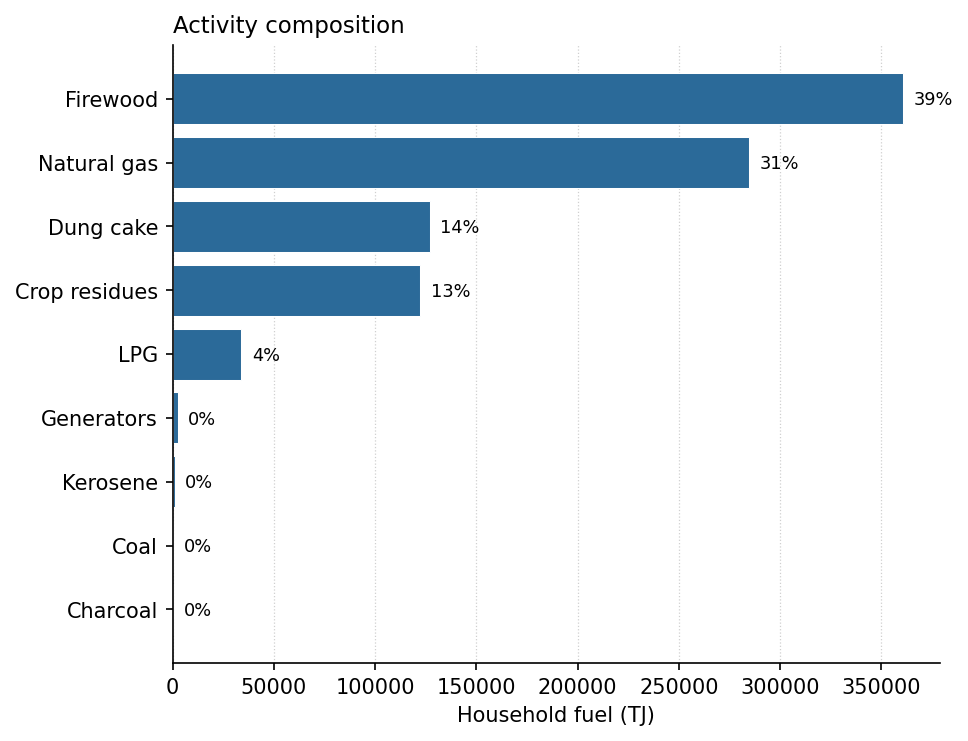
\includegraphics[width=\linewidth]{residential_activity.png}
\caption{Activity composition. Biomass---dung, firewood, crop residues and charcoal together---is \SI{65.4}{\percent} of
household energy, which is the fact behind both the particulate result and the sector's
uncertainty.}
\label{fig:activity}
\end{figure}

\subsection{The fossil streams}

Natural gas, LPG and kerosene are metered, billed and reported by the regulator with a domestic
sector breakdown. They are the best-constrained activity data in the sector and carry
correspondingly narrow uncertainties: \SI{10.8}{\percent} on gas \COtwo{},
\SI{20.9}{\percent} on LPG, \SI{20.2}{\percent} on kerosene.

Natural gas alone is \SI{15.96}{\mega\tonne} of \COtwo{}---\SI{66}{\percent} of the sector's
reported emissions from \SI{31}{\percent} of its energy---because it is the only major stream
whose \COtwo{} is reportable rather than a memo item.

\subsection{Dung cake: one diverted quantity, two destination readings}

The quantity agriculture diverts as dung fuel is derived from that sector's own nitrogen
flow: the same herd, the same species categories, the same burned-fuel shares that drive
agriculture's removal, converted from nitrogen to volatile solids at IPCC's rates for
the same animal categories and region (\ref{app:dung}). The chain runs
\SI{38.77}{\mega\tonne} of ash-free volatile solids $\rightarrow$ \SI{51.69}{} of
total dry solids (ash restored) $\rightarrow$ \SI{58.74}{\mega\tonne} of air-dry cake
(moisture restored, the mass the as-received calorific value pairs with; fractions from
proximate-analysis literature \citep{szymajda2019}; Table~\ref{tab:massbases}).

What that diverted mass does next is read two ways. The reference books to household
combustion the cake households report burning in HIES: the two rounds
(\SI{6.50}{\mega\tonne} in 2018--19, \SI{11.97}{} in 2024--25) anchor a per-household
quantity, interpolated between the rounds and held at the first round's rate before it,
and FY2023--24, which lies between them, takes \SI{10.93}{\mega\tonne}
(\SI{9.62}{} of total dry solids). The remainder's destination is left unresolved,
outside the total. Configuration L books all \SI{58.74}{\mega\tonne} to household
combustion: a destination assumption for the diverted dung, the reference of earlier
releases, and not a reading of household use. Section~\ref{sec:results} carries both.

The survey leaves its own questions open. The two rounds disagree by a factor of
\num{1.53} per household. The design SE of the dung total is \SI{6.6}{\percent} in
2024--25 and \SI{4.1}{} in 2018--19, and in 2024--25 the top 5\% of reporting
households hold \SI{44.7}{\percent} of the reported dung, against \SI{19.6}{} in
the earlier round. The dung activity term therefore carries \SI{35}{\percent}, the
width firewood carries.

\subsection{Firewood, measured by survey}

Firewood is the largest household fuel by energy and the only one with no
supply-side statistic. The quantity used here is the HIES 2024--25 design-weighted
national total \citep{hies2025}---\SI{23.1}{\mega\tonne} of air-dry wood a year entering
households as purchased, own-produced, in-kind or gifted consumption, recorded in kilograms
over a one-month recall for 30,123 households and weighted to the 39.9 million the sampling
frame represents.

One vintage mismatch is explicit rather than smoothed: the survey's field year is July 2024
to June 2025 (each household reporting one month within it), while this inventory's
reference year is FY2023--24. The round is applied to the adjacent fiscal year because it
is the nearest measurement---the alternative is the 2018--19 round, six years out---and
the two rounds' 6~percent agreement bounds what a one-year offset can plausibly move; the
offset is one of the systematic risks the stream's \SI{35}{\percent} uncertainty prices.
The time series (Section~\ref{sec:results}) interpolates per-household quantities between
the rounds rather than pinning either to a year it did not measure.

\begin{table}[htbp]
\centering
\footnotesize
\begin{tabular}{@{}lrr@{}}
\toprule
 & \textbf{2018--19} & \textbf{2024--25} \\
\midrule
Reporting households ($n$)          & 10\,636 & 11\,524 \\
Weighted user households (M)        & 13.0 & 14.0 \\
kg per user household per day       & 4.63 & 4.52 \\
Design SE of the total (\%)         & 2.4$^a$ & 7.1$^b$ \\
Top 1\% of households' share        & 0.05 & 0.19 \\
Top 5\% of households' share        & 0.17 & 0.33 \\
Interview quarters covered          & n/r & 4 of 4 \\
\bottomrule
\end{tabular}
\caption{Firewood survey diagnostics
(\texttt{hies\_diagnostics.csv}). Stratum-clustered linearized SEs: $^a$on the
published PSU; $^b$on an enumeration-block proxy (the 2024--25 release publishes no
PSU variable), so the two are not strictly comparable. The 2024--25 round's heavier
tail---one percent of reporting households carrying \SI{19}{\percent} of the weighted
total, against \SI{5}{} in 2018--19---is the single diagnostic most worth watching;
the per-user-day quantities, in the \SIrange{4.5}{4.6}{\kilo\gram} band both rounds,
are the reassuring one.}
\label{tab:hiesdiag}
\end{table}

Three estimates now bracket the quantity, and their agreement is the basis for trusting any
of them. The independent HIES 2018--19 round \citep{hies2019}, a different sample six years
earlier, gives \SI{22.0}{\mega\tonne}---within \SI{6}{\percent}. FAOSTAT's supply series
\citep{faostat}, the previous anchor for this stream, sits \SI{7}{\percent} above the
survey once its oven-dry basis is moisture-matched. A household self-report and a commodity
supply balance carry different biases, so their convergence is informative in a way
neither alone could be, and the comparison is a published output. FAOSTAT carries FAO's own ``E'' estimate flag in every year since 2009 and does not
move between years, which is why it was demoted to a structural scenario rather than retained
as the estimate.

Section~\ref{sec:results} still reports the sector three
additional ways---excluded, and at $\pm\SI{35}{\percent}$ quantity---so a reader can see
exactly what firewood is worth. The \SI{35}{\percent} carried in the propagation, down from
\SI{60}{\percent} in the FAOSTAT era, is not the survey's sampling error---the
stratum-clustered design SE is \SI{7.1}{\percent} for the 2024--25 round and
\SI{2.4}{} for 2018--19 (Table~\ref{tab:hiesdiag})---but prices what a household survey
cannot see: one-month recall scaled to a year, wood consumed outside the dwelling,
informal-enterprise use booked to households, and the outlier concentration the
diagnostics table quantifies.

\subsection{What is deliberately absent}

Household electricity. At \SI{39728}{\giga\watt\hour} it is the largest single item in every
Pakistani household energy statistic---nearly half of national consumption---and it is not in
this sector, because those emissions are generated at the power station and counted in 1A1a.
Adding them here would double-count roughly a quarter of the national inventory. A test asserts
that no electricity stream exists, so a future edit that "fixes the missing
electricity" is rejected rather than silently inflating the country's emissions.

Household coal and charcoal, once NE here, are now the sector's two smallest streams: the
HIES processing that re-anchored firewood measured them in passing, at \SI{13.2}{\kilo\tonne}
of coal and \SI{8.3}{\kilo\tonne} of charcoal---each reported by about one household in a
thousand, three orders of magnitude below firewood, and roughly a tenth of what the
2018--19 round recorded. With so few reporting households the survey \emph{suggests} a
substantial decline rather than confirms one: the clustered design SEs are
\SI{34}{\percent} on the 2024--25 coal total (23 reporting households, the heaviest
one percent of them carrying \SI{35}{\percent} of it) and \SI{16}{} on charcoal, and
questionnaire harmonisation between rounds has not been audited for these two items.
The decline direction survives intervals that wide; its magnitude does not. The regulator's
nil household coal figure turns out to be roughly right for the wrong reason: not silence,
but a quantity too small for a supply table to resolve. One residue caveat is carried in the conservative direction: the crop-residue stream
is an \emph{upper-bound residential allocation} of the agriculture-ledger fuel destination.
The ledger's fuel fraction covers all fuel use of each residue, not household fuel
specifically---brick kilns and small industry burn cotton sticks too---so
$R_{\text{fuel}} = R_{\text{household}} + R_{\text{commercial/industrial}} +
R_{\text{unresolved}}$, and booking the whole destination to households can only
overstate this sector. The survey's price bracket is the demand-side check that bounds
it, and the HIES expenditure items are the future constraint on the household share. What remains absent is biogas
(digester counts not obtained; NE) and the upstream wood carbonised into the charcoal
(roughly \SI{35}{}--\SI{50}{\kilo\tonne}, booked to the producing category IPCC assigns
it and unestimated nationally).
